% Meridian operator manual: how to run the interface and what every protocol step does.
% Overleaf: New Project > Upload Project > this file (or paste into main.tex). Compiler: pdfLaTeX.
% No other files are needed; figures are drawn with TikZ.
\documentclass[11pt,a4paper]{article}

\usepackage[T1]{fontenc}
\usepackage{lmodern}
\usepackage[margin=2.2cm]{geometry}
\usepackage{microtype}
\usepackage{booktabs}
\usepackage{array}
\usepackage{tabularx}
\usepackage{longtable}
\usepackage{enumitem}
\usepackage{xcolor}
\usepackage{tikz}
\usetikzlibrary{arrows.meta,positioning,fit,backgrounds}
\usepackage[most]{tcolorbox}
\usepackage{fancyhdr}
\setlength{\headheight}{14pt}
\usepackage[hidelinks]{hyperref}

\definecolor{ink}{HTML}{1F2A36}
\definecolor{clay}{HTML}{A8543A}
\definecolor{moss}{HTML}{3D6B45}
\definecolor{sky}{HTML}{2F5F8A}
\definecolor{sand}{HTML}{F3EDE3}
\definecolor{amber}{HTML}{C08A1E}

\hypersetup{colorlinks=true,linkcolor=sky,urlcolor=sky}
\setlist{itemsep=2pt,topsep=4pt}
\setlength{\parindent}{0pt}
\setlength{\parskip}{5pt}
\renewcommand{\arraystretch}{1.25}

\pagestyle{fancy}
\fancyhf{}
\lhead{\small\color{ink}Meridian operator manual}
\rhead{\small\color{ink}\nouppercase{\leftmark}}
\cfoot{\small\thepage}

\newcommand{\code}[1]{\texttt{\detokenize{#1}}}
\newcommand{\ui}[1]{\textsf{\textbf{#1}}}
\newcommand{\key}[1]{\fbox{\texttt{#1}}}

\newtcolorbox{stepbox}[1]{enhanced,breakable,colback=white,colframe=ink!40,coltitle=white,colbacktitle=ink,
  fonttitle=\bfseries,title={#1},boxrule=0.5pt,arc=2pt,left=6pt,right=6pt,top=4pt,bottom=4pt}
\newtcolorbox{tipbox}{enhanced,breakable,colback=moss!6,colframe=moss,boxrule=0.5pt,arc=2pt,left=6pt,right=6pt,
  title={Tip},fonttitle=\bfseries,colbacktitle=moss,coltitle=white}
\newtcolorbox{warnbox}{enhanced,breakable,colback=clay!6,colframe=clay,boxrule=0.5pt,arc=2pt,left=6pt,right=6pt,
  title={Important},fonttitle=\bfseries,colbacktitle=clay,coltitle=white}

% Step description: #1 participant sees, #2 operator does, #3 duration and advance, #4 data and purpose
\newcommand{\stepdetail}[4]{%
  \begin{tabularx}{\linewidth}{@{}>{\bfseries}p{3.3cm}X@{}}
    Participant sees & #1 \\
    Operator does & #2 \\
    Length / advances & #3 \\
    Data and purpose & #4 \\
  \end{tabularx}}

\title{\color{ink}\textbf{Meridian Multimodal Research Platform}\\[6pt]
  \Large Operator manual: running the interface and the study protocol step by step}
\author{Your Name \\ IIT Ropar}
\date{Protocol v9 \quad\textbar\quad \today}

\begin{document}
\maketitle
\thispagestyle{empty}

\begin{abstract}
This manual explains how to install, start, and operate Meridian, the lab system that records a participant
with contact and contactless sensors while they watch emotional film clips, answer questionnaires, perform
cognitive tasks, and follow breathing and movement instructions. Part I covers the hardware and software setup
and how to prepare a session. Part II walks through every step of the study protocol: what the participant
sees, what the operator does, how long it takes, and what data it produces. Part III covers ending a session,
reading the quality report, do's and don'ts, and troubleshooting.
\end{abstract}

\tableofcontents
\newpage

% =====================================================================
\part{Setting up and starting a session}
% =====================================================================

\section{What Meridian is}

Meridian has three parts that work together during a recording.

\begin{center}
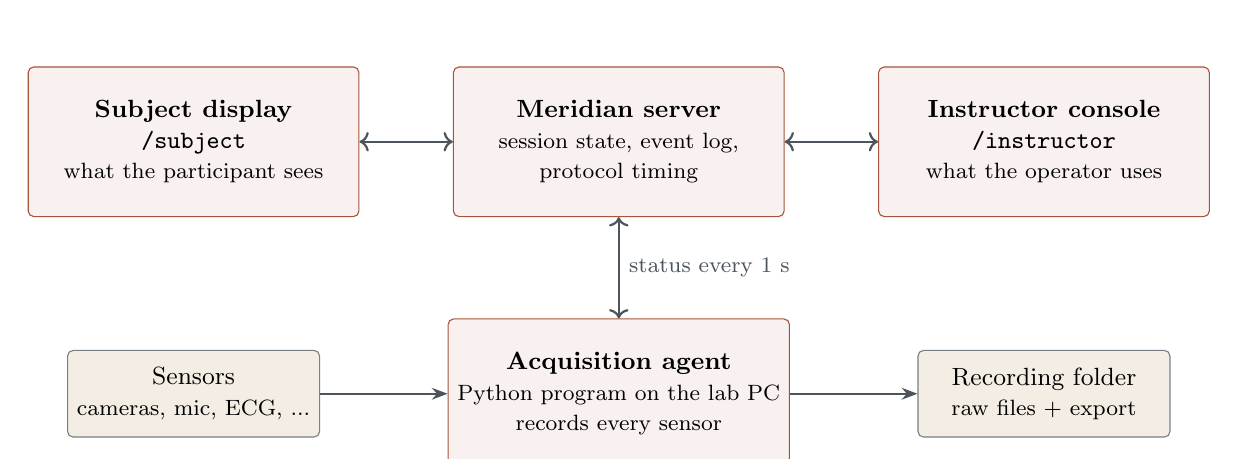
\begin{tikzpicture}[font=\small,
  comp/.style={draw=clay,fill=clay!8,rounded corners=2pt,align=center,minimum width=4.2cm,minimum height=1.9cm},
  store/.style={draw=ink!60,fill=sand,rounded corners=2pt,align=center,minimum width=3.2cm,minimum height=1.1cm},
  arr/.style={-{Stealth[length=2mm]},thick,ink!80}]
  \node[comp] (sub) at (0,0) {\textbf{Subject display}\\\code{/subject}\\\footnotesize what the participant sees};
  \node[comp] (srv) at (5.4,0) {\textbf{Meridian server}\\\footnotesize session state, event log,\\\footnotesize protocol timing};
  \node[comp] (ins) at (10.8,0) {\textbf{Instructor console}\\\code{/instructor}\\\footnotesize what the operator uses};
  \node[comp] (agt) at (5.4,-3.2) {\textbf{Acquisition agent}\\\footnotesize Python program on the lab PC\\\footnotesize records every sensor};
  \node[store] (sens) at (0,-3.2) {Sensors\\\footnotesize cameras, mic, ECG, ...};
  \node[store] (disk) at (10.8,-3.2) {Recording folder\\\footnotesize raw files + export};
  \draw[arr,<->] (sub) -- (srv);
  \draw[arr,<->] (ins) -- (srv);
  \draw[arr,<->] (agt) -- node[right,font=\footnotesize]{status every 1 s} (srv);
  \draw[arr] (sens) -- (agt);
  \draw[arr] (agt) -- (disk);
\end{tikzpicture}
\end{center}

\begin{description}
  \item[Subject display] A browser page on the participant's screen. It shows one instruction or task at a time:
    clips, rating scales, questionnaires, the Stroop and N-back tasks, breathing guides, and resting screens.
  \item[Instructor console] A browser page for the operator. It is used to set up the session (devices, consent,
    screening, participant details), watch every sensor live, start, pause, and advance the protocol, and label
    disturbances.
  \item[Acquisition agent] A Python program on the lab computer. It opens every sensor, streams live status to the
    console, records raw data to disk with timestamps on one clock, and writes the analysis bundle at the end.
\end{description}

A finished session produces a folder with one raw file per sensor (lossless video, audio, CSV signals), an event log
of everything that happened in the protocol, and an \code{export/} bundle with tables, derived signals, a BIDS-style
copy, and a quality-assurance (QA) report.

\section{One-time installation}

\subsection{Web application}
On the lab computer, in the repository folder:
\begin{verbatim}
cd /media/ai/OneTB/aarush_new_interface
npm install          # once, installs the web application
npm run dev          # starts the server on http://localhost:3000
\end{verbatim}
Keep the server running for the whole session. Open the pages on the same computer:
\code{http://localhost:3000/instructor} and \code{http://localhost:3000/subject}.

\subsection{Acquisition agent}
The agent needs Python 3.11 or newer with the packages in \code{acquisition_agent/requirements.txt}
(pyserial, OpenCV, sounddevice, websocket-client, NumPy):
\begin{verbatim}
cd acquisition_agent
python3 -m pip install -r requirements.txt
\end{verbatim}
On Linux the user must be in the \code{dialout} group (serial sensors) and the \code{video} group (cameras).

\subsection{Stable device names}
Linux renumbers devices (\code{/dev/video0}, \code{/dev/ttyUSB1}) every time they are replugged. Always assign
devices by their stable names, which never change:
\begin{itemize}
  \item cameras: \code{/dev/v4l/by-id/usb-...-video-index0}
  \item serial boards: \code{/dev/serial/by-id/usb-...}
  \item audio: the device name, for example \code{ILCE-6700}
\end{itemize}
The device lists in the instructor console already show these names.

\section{Hardware setup}

\subsection{Devices}
\begin{longtable}{@{}p{3.2cm}p{4.3cm}p{2.1cm}p{5.6cm}@{}}
\toprule
\textbf{Stream} & \textbf{Device and connection} & \textbf{Rate} & \textbf{Why it is recorded} \\
\midrule\endhead
Face camera 1 & Logitech BCC950, USB directly to the PC & 30 fps, 640x480 & Camera heart rate (rPPG), facial expression; uncompressed input, exposure locked \\
Face camera 2 & Sony a6700 in USB Streaming mode, 720p & 25 fps, 1280x720 & Second, sharper face view \\
Audio & DJI Mic Mini, two transmitters into one receiver in the Sony mic jack; recorded from the Sony USB audio & 48 kHz, 2 channels & Speech during conversation and movement steps; voice arousal. Mic 1 on the participant (left channel), mic 2 on the operator (right channel) \\
Thermal camera & FLIR UVC camera & about 10 fps & Facial skin temperature, breathing at the nostrils \\
ECG & Frontier X chest strap, live share link from the phone app & 125 Hz & Reference heart rate and heart-rate variability \\
Pulse oximeter & CMS50E, USB serial & 60 Hz & Heart rate, SpO2, fingertip pulse wave \\
EDA / GSR & ESP32 skin-conductance board, USB serial & 20 Hz & Sympathetic arousal (sweat response) \\
WiFi CSI & ESP32 receiver on USB; ESP32 transmitter on a powerbank & 100 Hz & Contactless breathing and heart signals \\
Optional & EMG, respiration belt, photodiode, room environment, second CSI receiver & various & Muscle activity, breathing reference, display timing, room conditions \\
\bottomrule
\end{longtable}

\subsection{Rules for connecting}
\begin{itemize}
  \item Plug \textbf{cameras directly into rear USB ports} of the PC. Do not put cameras on an unpowered USB 2.0 hub;
    during testing such a hub reset itself and stopped both cameras.
  \item Put serial boards (oximeter, GSR, CSI, and other ESP32 boards) on a \textbf{powered} USB hub.
  \item Boards with electrodes on the body (GSR, EMG) should go through a USB isolator or run on batteries.
  \item The CSI transmitter only needs power; a powerbank is fine.
  \item Only \textbf{one program} may use a serial port. Close other dashboards that read the ESP32.
\end{itemize}

\subsection{Camera and room settings}
\begin{itemize}
  \item Sony a6700: Menu, Setup, USB Streaming on; output resolution \textbf{720p}. At 1080p/50 fps the PC dropped
    38\,\% of frames. Set exposure, ISO, and white balance \textbf{manually}; the camera ignores the software lock.
  \item Fixed lighting (lights on, blinds closed), door closed, phones silent, nobody walking behind the participant.
  \item Participant seated 50 to 80 cm from the cameras, face centred in both previews.
  \item Disk: a full session with two lossless cameras and thermal uses about 75 GB.
\end{itemize}

\section{Starting the software}

\subsection{Step 1: create a session}
In the instructor console, create a session with the participant number. Meridian gives it a code such as
\code{9997VFQB}. The participant number sets the order of the emotions and tasks (Section~\ref{sec:counterbalancing}).

\subsection{Step 2: start the acquisition agent}
The console shows the exact command under \ui{Recording setup}, \ui{Technical connection}. Run it in a terminal on the
lab PC, adding the second camera and audio device:
\begin{verbatim}
cd /media/ai/OneTB/aarush_new_interface/acquisition_agent
python3 -m meridian_agent --server http://localhost:3000 \
  --code SESSIONCODE --token SESSIONTOKEN \
  --camera /dev/v4l/by-id/usb-046d_BCC950_...-video-index0 \
  --camera2 /dev/v4l/by-id/usb-Sony_ILCE-6700_...-video-index0 \
  --audio ILCE-6700 --audio-channels stereo
\end{verbatim}
The other devices (oximeter, GSR, ECG link, thermal, CSI) can be passed as flags or assigned in the console.

\ui{--audio-channels stereo} keeps the two microphones on separate channels. Without it the agent averages them to
one track and the participant can no longer be separated from the operator, which cannot be undone afterwards. The
flag is not settable from the console, so it has to be on this command line every session.

\begin{warnbox}
Run only \textbf{one agent at a time}. Two agents fight for the same cameras and ports and both recordings are
damaged. Stop the old agent (Ctrl+C) before starting one for a new session. The agent exits by itself after a
session is finalized.
\end{warnbox}

\subsection{Step 3: open the two pages}
\begin{enumerate}
  \item Instructor console: \code{http://localhost:3000/instructor}, open the session. \textbf{Keep this tab open
    for the whole session}; if the console is not seen for 12 seconds the session pauses automatically.
  \item Subject display on the participant screen: \code{http://localhost:3000/subject}, type the session
    \textbf{code} (not the participant number), press \ui{CONNECT}. It downloads all clips before the session can start.
\end{enumerate}

\section{Preparing the session in the instructor console}

Open \ui{Recording setup}. Every section saves automatically and shows \ui{Saved}, \ui{Saving...} or
\ui{Not saved yet}. Entries are kept even if the dialog is closed or the page is reloaded. Fields marked
\textbf{*} are required.

\subsection{Recording devices and required streams}
For each stream choose the device and tick \ui{Require} for streams the session cannot run without. Recommended
required set: face camera 1, face camera 2, audio, pulse oximeter, GSR, ECG. Thermal and CSI can stay optional.
Press \ui{SAVE RECORDING SETUP}. A device that is not in the list keeps its current value (shown as
\ui{Current: ...}).

\subsection{Protocol options}
\begin{tabularx}{\linewidth}{@{}lX@{}}
\toprule
Questionnaires & PANAS mood at start and end, TIPI personality at start, NASA-TLX workload after Stroop and N-back \\
Paced breathing & 60 s each at 6, 10, 15 and 20 breaths per minute \\
Longer exertion & 60 s instead of 20 s \\
Neutral control clip & Neutral clip, rating and washout before Part 1 (only if a neutral clip is registered) \\
Continuous rating replay & All clips replayed at the end with a continuous valence-arousal marker (off by default; adds about 15 min) \\
\bottomrule
\end{tabularx}

\subsection{Consent (*)}
Record what the signed consent form allows. Only \textbf{participation} is required; every sharing question left
unanswered is saved as \textbf{No}, the most private choice. The share manifest in the export uses these answers to
mark each file shareable or withheld.

\subsection{Safety screening (*)}
Ask all six questions. A \textbf{Yes} automatically skips the related physical steps.
\begin{longtable}{@{}p{8.8cm}p{5.8cm}@{}}
\toprule
\textbf{Question} & \textbf{A yes skips} \\
\midrule\endhead
Any heart condition, chest pain, or blood pressure condition under treatment? & Breath hold, exertion \\
Asthma, COPD, or another breathing condition? & Breath hold, exertion \\
History of fainting, or dizziness when standing up? & Standing \\
An injury or condition that makes standing up or marching in place difficult? & Standing, exertion \\
Currently pregnant? & Breath hold, exertion \\
Unwell today, or advised by a doctor to avoid exercise? & Breath hold, exertion \\
\bottomrule
\end{longtable}

\subsection{Participant details}
Categories only; never names or dates. Required (*): skin type (Fitzpatrick I to VI, use the reference card),
age band, sex, eyewear. Optional but useful: handedness, BMI band, facial hair, makeup, caffeine, nicotine, or exercise in
the last two hours, medication affecting heart rate, and camera distances. Skin type and eyewear strongly affect camera
and thermal signals.

\subsection{WiFi CSI setup and empty-room baseline (optional)}
Enter channel, bandwidth, packet rate, and the positions of transmitter, receiver, and participant. Before the
participant sits down, with nobody in the room, press \ui{RECORD EMPTY ROOM} (60 s). This baseline lets analysis
separate the person from the room.

\subsection{Put the sensors on}
\begin{enumerate}
  \item \textbf{ECG strap}: wet the electrodes, strap snug under the chest; start live streaming in the Frontier X
    app; keep the phone awake and charging.
  \item \textbf{Pulse oximeter}: index finger of the non-dominant hand, hand resting on the table.
  \item \textbf{GSR electrodes}: two fingers of the same hand, skin clean and dry; allow about 5 minutes to settle.
  \item \textbf{DJI Mic Mini}: both transmitters switched on. \textbf{Mic 1 on the participant}, clipped near the
    collar; \textbf{mic 2 on the operator}. Mic 1 is the left channel and mic 2 the right, so swapping them puts the
    operator's voice in the participant's channel for the whole session.
  \item \textbf{Seating}: face centred in both camera previews, hair off the forehead.
\end{enumerate}

\textbf{Signal targets before starting} (Overview tab):
\begin{tabularx}{\linewidth}{@{}lX@{}}
\toprule
ECG & heart rate plausible, about 50 to 100 bpm at rest \\
Pulse oximeter & finger detected; heart rate within 8 bpm of the ECG (heart-rate agreement card) \\
GSR & above 0.5 uS and fairly stable (0.00 uS means no skin contact) \\
Face cameras & face visible in both previews, 0 dropped frames \\
Audio & level meter moves when the participant speaks; with two mics, check each channel separately using \texttt{tools/audio\_check.py} \\
\bottomrule
\end{tabularx}

\subsection{Preflight}
Press \ui{RUN PREFLIGHT}. For 10 seconds the agent checks that every required stream delivers good data, that local
storage is writable with enough free space, and that the clocks agree (offset below 100 ms). Run it again after any
hardware change.

\subsection{The start checklist}
Below \ui{START SESSION} the console lists every requirement with a tick or a cross and the reason. The server
refuses to start until all are ticked.

\begin{longtable}{@{}p{3.6cm}p{5cm}p{6cm}@{}}
\toprule
\textbf{Check} & \textbf{Passes when} & \textbf{How to fix a cross} \\
\midrule\endhead
Consent & Participation is Yes and saved & Open Consent, choose participation \\
Safety screening & All six answers saved & Answer every question \\
Acquisition agent & Agent reported in the last 10 s & Start the agent with this session's code and token \\
Required devices assigned & Every required stream has a device & Assign a device, or untick Require \\
Required streams live & Every required stream sends good data & Fix the sensor named in the message \\
Preflight & Last preflight passed & Run preflight after fixing the streams \\
Subject display & All clips loaded & Open \code{/subject}, enter the session code \\
\bottomrule
\end{longtable}

When everything is ticked, press \ui{START SESSION}. Recording begins immediately for every stream.

% =====================================================================
\part{The study protocol step by step}
% =====================================================================

\section{Overview of the protocol}

The default protocol (v9) has \textbf{43 steps} and takes about \textbf{50 minutes}. With the optional continuous
rating replay it has 49 steps and takes about 65 minutes.

\begin{center}
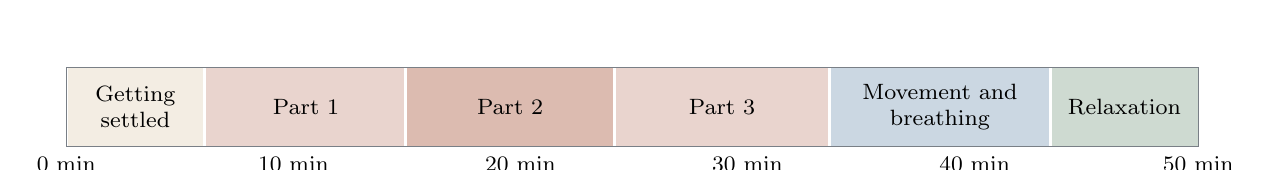
\begin{tikzpicture}[x=0.0048cm,y=1cm,font=\footnotesize]
  \foreach \start/\len/\name/\col in {0/365/Getting settled/sand, 365/531/Part 1/clay!25, 896/552/Part 2/clay!40,
      1448/568/Part 3/clay!25, 2016/585/Movement and breathing/sky!25, 2601/390/Relaxation/moss!25}{
    \pgfmathsetmacro{\phasemid}{\start+\len/2}
    \pgfmathsetmacro{\phasewidth}{\len*0.0044}
    \fill[\col] (\start,0) rectangle ++(\len,1);
    \draw[white,line width=1pt] (\start,0) -- ++(0,1);
    \node[align=center,text width=\phasewidth cm] at (\phasemid,0.5) {\name};
  }
  \draw[ink!60] (0,0) rectangle (2991,1);
  \foreach \t/\m in {0/0,600/10,1200/20,1800/30,2400/40,2991/50} \node[below] at (\t,0) {\m\ min};
\end{tikzpicture}
\end{center}

\subsection{How steps advance}
\begin{tabularx}{\linewidth}{@{}lX@{}}
\toprule
\textbf{Type} & \textbf{Meaning} \\
\midrule
Operator & Waits for the operator to press \ui{ADVANCE} \\
Task & Advances when the participant finishes the questionnaire, rating, or task \\
Timer & Advances when the timer ends (pause time is not counted); the operator can press \ui{ADVANCE} early \\
Media & Advances when the clip finishes playing \\
Gate & Waits until heart rate and skin conductance have returned to baseline, or the operator overrides with a reason \\
Subject & The participant ends the step (breath hold) \\
\bottomrule
\end{tabularx}

\subsection{Counterbalancing}\label{sec:counterbalancing}
Six emotions are shown in pairs across three parts. The \textbf{emotion order} comes from a six-row Williams square,
row $= (\mathit{participant}-1) \bmod 6$, so each emotion follows every other emotion equally often. The \textbf{task
order} (Stroop, N-back, conversation) comes from an independent row $= \lfloor(\mathit{participant}-1)/6\rfloor \bmod 6$,
so 36 participants cover every pairing of emotion order and task order.

\begin{center}
\small
\begin{tabular}{@{}cl@{}}
\toprule
Row & Emotion order \\
\midrule
1 & happy, sad, disgust, anger, surprise, fear \\
2 & sad, anger, happy, fear, disgust, surprise \\
3 & anger, fear, sad, surprise, happy, disgust \\
4 & fear, surprise, anger, disgust, sad, happy \\
5 & surprise, disgust, fear, happy, anger, sad \\
6 & disgust, happy, surprise, sad, fear, anger \\
\bottomrule
\end{tabular}
\end{center}

The step descriptions below use participant 1 (row 1: happy, sad, disgust, anger, surprise, fear; tasks Stroop,
N-back, conversation). Other participants see the same step types with the emotions and tasks rotated. A cognitive task
(Stroop or N-back) is followed by a NASA-TLX workload rating; the conversation is not.

\subsection{Rules that hold for every step}
\begin{itemize}
  \item Every step start, end, clip onset, answer, and pause is written to the event log with a timestamp on the
    recording clock, so it can be aligned with every sensor sample.
  \item The subject display records when each step actually appeared on screen.
  \item A pause freezes the step timer and the clip; resuming continues where it stopped.
\end{itemize}

% ---------------------------------------------------------------------
\section{Phase 1: Getting settled (about 6 minutes)}

\begin{stepbox}{Step 0 -- Sensor and synchronization check}
\stepdetail{``Look toward the screen and stay still.''}
{Checks that every required stream is green in the Overview and the heart-rate agreement card agrees, then presses
\ui{ADVANCE}.}
{About 30 s; operator advances.}
{A short still segment at the very start of every recording; confirms synchronization before any stimulus.}
\end{stepbox}

\begin{stepbox}{Step 1 -- Current mood questionnaire (PANAS, start)}
\stepdetail{20 mood words (for example interested, distressed, excited), one at a time, each on a 5-point scale from
``very slightly or not at all'' to ``extremely''.}
{Says: ``Please answer each question on the screen. There are no right or wrong answers.'' Stays quiet.}
{About 75 s; advances when all items are answered.}
{Positive and negative affect scores before any stimulus; compared with the end-of-session PANAS.}
\end{stepbox}

\begin{stepbox}{Step 2 -- Personality questionnaire (TIPI)}
\stepdetail{10 statements, one at a time, on a 7-point scale from ``disagree strongly'' to ``agree strongly''.}
{Stays quiet.}
{About 50 s; advances when done.}
{Big Five personality scores, used to explain individual differences in emotional responses.}
\end{stepbox}

\begin{stepbox}{Step 3 -- Resting baseline, eyes open}
\stepdetail{A fixation cross. ``Look at the cross. Breathe naturally.''}
{Says: ``Look at the cross and breathe normally.'' Keeps the room silent. Enters a resting blood-pressure reading if
a cuff is used.}
{120 s; timer.}
{Resting reference for every physiological signal. Heart rate and skin conductance samples after the first 15 s
build the baseline that the return-to-baseline gates use later.}
\end{stepbox}

\begin{stepbox}{Step 4 -- Resting baseline, eyes closed}
\stepdetail{``Close your eyes. Breathe naturally.''}
{Says: ``Gently close your eyes and keep breathing naturally.'' Silence.}
{90 s; timer.}
{Eyes-closed resting reference (no visual input, fewer blinks).}
\end{stepbox}

% ---------------------------------------------------------------------
\section{Phases 2 to 4: the three emotion parts (about 9 to 10 minutes each)}

Each part follows the same pattern: \textbf{clip, rating, washout, clip, rating, activity, gate}.

\begin{stepbox}{Emotion clip (steps 5, 8, 13, 16, 21, 24)}
\stepdetail{A film clip chosen to evoke one emotion, full screen with sound. ``Watch naturally.''
Clip lengths: happy 93 s, fear 95 s, sad 148 s, anger 151 s, disgust 151 s, surprise 183 s.}
{Says: ``Watch the clip naturally and react however feels natural. There is no right or wrong response.'' Stays
out of view and silent. Presses a hotkey for any disturbance.}
{Clip length plus a few seconds; advances when the clip ends.}
{The emotional stimulus. Onset is logged when playback actually starts, offset when it ends; clips are loudness
normalized to the same level (-23 LUFS) and resolution (1280x720, 30 fps).}
\end{stepbox}

\begin{stepbox}{Self-report rating after each clip (steps 6, 9, 14, 17, 22, 25)}
\stepdetail{Six questions: 9-point valence (unpleasant to pleasant), arousal (calm to excited), and dominance
(controlled to in control); the main emotion felt; its intensity; whether the clip was seen before.}
{Says: ``Choose the response that best matches your experience. Go with your first instinct.''}
{About 40 s; advances when all six are answered.}
{Ground-truth labels for emotion recognition, per clip. Familiarity lets analysis exclude clips already known.}
\end{stepbox}

\begin{stepbox}{Neutral washout (steps 7, 15, 23)}
\stepdetail{A fixation cross, no instruction text.}
{Says: ``Rest your eyes on the cross and breathe normally.''}
{20 s; timer.}
{Separates the two clips of a part so the first emotion fades before the second begins.}
\end{stepbox}

\begin{stepbox}{Stroop colour-word task (step 10 for participant 1)}
\stepdetail{A colour word (for example RED) printed in an ink colour. The participant presses the button for the
\textbf{ink colour}, not the word. 30 trials: 15 congruent (word matches ink) and 15 incongruent, never more than three of
the same kind in a row, 400 ms fixation before each word, 2 s to respond.}
{Says: ``Select the button matching the ink colour, not what the word says. Respond as quickly and accurately as you
can.'' Does not help.}
{About 90 s; advances when all trials are done.}
{Cognitive load and interference: per-trial reaction time and accuracy, and the interference cost (incongruent
minus congruent reaction time). Physiology during the task shows mental effort.}
\end{stepbox}

\begin{stepbox}{N-back task (step 18 for participant 1)}
\stepdetail{A square appears in one of nine positions, one after another. The participant presses \ui{Match} when the
position is the same as N steps earlier. First a practice block of 8 trials with feedback, then 20 scored trials
with exactly 30\,\% targets.}
{Says: ``Press Match whenever the current position is the same as the position from N steps ago.'' Sets the N level
(1 to 3) in the Protocol tab before the task if the study requires it. Does not help.}
{About 50 s plus practice; advances when done.}
{Working-memory load: hits, misses, false alarms, reaction times, and sensitivity ($d'$).}
\end{stepbox}

\begin{stepbox}{Workload rating, NASA-TLX (after Stroop and after N-back)}
\stepdetail{Six scales from 0 to 100 in steps of 5: mental demand, physical demand, temporal demand, performance,
effort, frustration.}
{Stays quiet.}
{About 45 s; advances when done.}
{The participant's own rating of how demanding the task was; paired with performance and physiology for stress
and cognitive-load analysis.}
\end{stepbox}

\begin{stepbox}{Conversation (step 26 for participant 1)}
\stepdetail{``Talk together about something familiar.''}
{Talks with the participant for three minutes about a recent trip, a hobby, or how the day has been. This is the
\textbf{only step where talking is intended}, so there is no need to press \key{T} (talking) here.}
{180 s; timer.}
{Natural speech, facial movement, and social engagement: a realistic but low-stress condition for voice and video
analysis, and a test of contactless signals during speech.}
\end{stepbox}

\begin{stepbox}{Return-to-baseline gate (steps 12, 20, and 27)}
\stepdetail{``Sit quietly and breathe normally.''}
{Watches the gate panel in the Protocol tab. When it shows \ui{Returned to baseline}, presses \ui{ADVANCE}. If it
does not settle (for example skin conductance drifting), advances with an override and writes the reason.}
{At least 40 s; advances when the gate passes or is overridden.}
{Prevents one condition from carrying into the next. The gate passes when heart rate and skin conductance are within
the larger of two standard deviations of the resting baseline or a floor (5 bpm, 10\,\% of skin conductance) and
stay there for 15 s. The outcome (verified, not measurable, or overridden) is logged.}
\end{stepbox}

% ---------------------------------------------------------------------
\section{Phase 5: Movement and breathing (about 10 minutes)}

This phase deliberately changes breathing and heart rate so contactless estimates (camera, thermal, WiFi CSI) can be
validated against the contact references across a wide range, and adds known motion and speech artifacts.

\begin{stepbox}{Step 28 -- Seated rest}
\stepdetail{``Sit comfortably and stay still.''}
{Silence.}
{20 s; timer.}
{Short still anchor before the breathing exercises.}
\end{stepbox}

\begin{stepbox}{Step 29 -- Box breathing}
\stepdetail{A circle: breathe in as it grows, hold, breathe out as it shrinks, hold again.}
{Says: ``Breathe in as the circle grows, hold, breathe out as it shrinks, then hold again.''}
{45 s; timer.}
{Slow, regular breathing with pauses; a clear breathing pattern for respiration estimation.}
\end{stepbox}

\begin{stepbox}{Steps 30 to 33 -- Paced breathing at 6, 10, 15, and 20 breaths per minute}
\stepdetail{A bar that rises (breathe in) and falls (breathe out) at the set rate.}
{Says: ``Follow the guide. Breathe gently; do not force it.'' Watches for discomfort, especially at 6 per minute.}
{60 s each; timer.}
{Known breathing rates as ground truth. In testing, the belt measured 6.1 and 19.9 and WiFi CSI 5.9 and 20.0 breaths
per minute for the 6 and 20 per minute guides.}
\end{stepbox}

\begin{stepbox}{Step 34 -- Breath hold (skipped if screened out)}
\stepdetail{``Breathe in and hold. Release whenever you need to.''}
{Says: ``Take a normal breath in and hold only for as long as feels comfortable.'' Watches the participant.}
{Until the participant releases; limited to 60 s.}
{A strong, brief change in heart rate and oxygen saturation; tests how quickly each sensor follows.}
\end{stepbox}

\begin{stepbox}{Step 35 -- Head movement and speaking}
\stepdetail{``Turn left. Turn right. Look up. Look down. Then speak.''}
{Demonstrates if needed.}
{30 s; timer.}
{Controlled motion and speech artifacts, labelled by the protocol itself, for testing artifact robustness.}
\end{stepbox}

\begin{stepbox}{Step 36 -- Standing (skipped if screened out)}
\stepdetail{``Stand up slowly. Stay still.''}
{Says: ``Stand up slowly and remain still. Tell me immediately if you feel dizzy.'' Stands close by. Enters a standing
blood-pressure reading if a cuff is used.}
{45 s; timer.}
{Posture change raises heart rate (orthostatic response).}
\end{stepbox}

\begin{stepbox}{Step 37 -- Brief exertion (skipped if screened out)}
\stepdetail{``March in place or do sit-to-stands.''}
{Encourages a comfortable pace; stops the step if the participant is unwell.}
{60 s; timer.}
{Raises heart rate well above rest (72 to about 108 bpm in testing) for validating heart-rate estimates at high
rates, and adds strong motion for EMG.}
\end{stepbox}

\begin{stepbox}{Step 38 -- Post-exertion recovery}
\stepdetail{``Sit down. Stay still.''}
{Says: ``Sit back down and stay still while your breathing settles.'' Enters a post-exertion blood-pressure reading if
used.}
{60 s; timer.}
{Recovery curve of heart rate and breathing back toward rest.}
\end{stepbox}

% ---------------------------------------------------------------------
\section{Phase 6: Relaxation and end (about 6 minutes)}

\begin{stepbox}{Step 39 -- Guided body scan}
\stepdetail{``Get comfortable. Close your eyes.'' Guided audio.}
{Silence; dims attention away from the participant.}
{240 s; timer.}
{Deep relaxation condition: low arousal reference at the end of the session.}
\end{stepbox}

\begin{stepbox}{Step 40 -- Return to normal}
\stepdetail{``Open your eyes when you are ready.''}
{Enters a final blood-pressure reading if used.}
{60 s; timer.}
{Final eyes-open rest.}
\end{stepbox}

\begin{stepbox}{Step 41 -- Current mood questionnaire (PANAS, end)}
\stepdetail{The same 20 mood words as step 1.}
{Stays quiet.}
{About 75 s; advances when done.}
{Change in positive and negative affect across the whole session.}
\end{stepbox}

\begin{stepbox}{Optional: continuous rating replay (steps 42 to 47 when enabled)}
\stepdetail{Each clip plays again with a two-dimensional grid: left to right is unpleasant to pleasant, bottom to top
is calm to excited. ``Watch again and keep the marker where your feeling is.''}
{Explains the grid once, then stays quiet.}
{Each clip's length; advances when the clip ends.}
{Moment-by-moment valence and arousal sampled 20 times per second, for time-resolved emotion labels. Done at the end so
hand movement does not disturb the main recording.}
\end{stepbox}

\begin{stepbox}{Last step -- Session complete}
\stepdetail{``Thank you.''}
{Ends the session (Section~\ref{sec:ending}).}
{About 15 s; operator.}
{Marks the end of the protocol.}
\end{stepbox}

% ---------------------------------------------------------------------
\section{Operating during the recording}

\subsection{Controls}
\begin{tabularx}{\linewidth}{@{}lX@{}}
\toprule
\ui{PAUSE / RESUME} & Pause for anything unplanned (bathroom, discomfort, a sensor falling off). Sensors keep recording;
the protocol and clip stop. Resume only when signals are good again. \\
\ui{ADVANCE} & End the current step early (timers, operator steps, gates). \\
Gate override & In the Protocol tab, advance a gate that has not settled; a written reason is required. \\
Blood pressure & Enter readings during baseline, standing, recovery, and return to normal if a cuff is used. \\
N-back level & Set the N level (1 to 3) before the N-back step. \\
Subject message & Send a short instruction to the subject screen. \\
\bottomrule
\end{tabularx}

\subsection{Artifact hotkeys}
Press these in the instructor console the moment something happens. They are exported to \code{artifacts.tsv} and
excluded from quality statistics.

\begin{tabularx}{\linewidth}{@{}clX@{}}
\toprule
\textbf{Key} & \textbf{Label} & \textbf{How it works} \\
\midrule
\key{T} & Talking & Press to start, press again to end \\
\key{L} & Left seat & Press to start, press again to end \\
\key{O} & Operator in view & Press to start, press again to end \\
\key{C} & Cough or sneeze & Marks the last 3 seconds \\
\key{M} & Large movement & Marks the last 3 seconds \\
\key{D} & Door or other people & Marks the last 3 seconds \\
\key{P} & Phone & Marks the last 3 seconds \\
\bottomrule
\end{tabularx}

\subsection{Automatic pauses}
The server pauses the session and logs why when:
\begin{itemize}
  \item the instructor console has not been seen for 12 seconds (tab closed or computer asleep);
  \item a required stream stops while recording (after a short start-up grace period).
\end{itemize}
Fix the cause, then press \ui{RESUME}.

\subsection{Safety}
Stop the physical steps at once if the participant reports dizziness, chest discomfort, breathlessness, or feels
unwell. Pause the session, attend to the participant, and note what happened. The participant's wellbeing always comes
before the recording.

% =====================================================================
\part{After the session}
% =====================================================================

\section{Ending the session and the data}\label{sec:ending}

\subsection{Ending}
\begin{enumerate}
  \item At the last step (or to stop early) press \ui{END SESSION}.
  \item Wait until the agent reports that the analysis bundle is written (1 to 3 minutes). Do not unplug devices or
    close the agent before then.
  \item Remove the sensors and thank the participant.
\end{enumerate}

\subsection{Recording folder}
\begin{verbatim}
.local-run/recordings/session_CODE_DATE_TIME/
  face/face.mkv  face/face_frames.csv        lossless video + frame times
  face2/face2.mkv  face2/face2_frames.csv
  thermal/thermal.mkv  audio/audio.wav
  ecg/ecg.csv  oximeter/oximeter.csv  gsr/gsr.csv  csi/csi.csv
  session_events.jsonl  manifest.json  acquisition.json
  export/
    qa_report.md  qa_report.json  events.tsv  steps.tsv
    ratings.tsv  tasks.tsv  stroop_trials.tsv  nback_trials.tsv
    questionnaire_items.tsv  questionnaire_scores.tsv
    annotations.tsv  artifacts.tsv  participants.tsv
    consent.json  share_manifest.json  session.json
    derivatives/physio_summary.tsv  derivatives/ecg_rpeaks.tsv.gz
    bids/
\end{verbatim}
Every sensor row carries \code{host_epoch_ns}, the same clock used for protocol events.

\subsection{Reading the QA report}
Open \code{export/qa_report.md}. It lists, per step, the active and planned time, coverage of each required stream,
pauses, and restarted clips; and per session, skipped steps, gate outcomes, missing participant details, CSI
baseline, and the display timing check.

\begin{tabularx}{\linewidth}{@{}lX@{}}
\toprule
\textbf{Check} & \textbf{Good result} \\
\midrule
Coverage & At least 95\,\% for every required stream in every step \\
Face videos & Frame count in the video equals the rows in \code{*_frames.csv}; dropout below 1\,\% \\
ECG vs oximeter & Heart rates within a few bpm in \code{physio_summary.tsv} \\
GSR & Above 0 uS throughout \\
Audio & Clear speech during the conversation step \\
Gates & Verified rather than overridden \\
Pauses & Only those you intended \\
\bottomrule
\end{tabularx}

\section{Do's and don'ts}

\begin{minipage}[t]{0.48\linewidth}
\begin{tipbox}
\textbf{Do}
\begin{itemize}[leftmargin=*]
  \item Keep the instructor console open all session.
  \item Mark every disturbance with a hotkey at once.
  \item Keep lighting, camera position, and Sony settings fixed.
  \item Keep the Frontier X phone awake and charging.
  \item Ask the participant to keep the sensor hand still.
  \item Pause for anything unplanned.
  \item Check signal targets before starting.
  \item Stop at once if the participant feels unwell.
\end{itemize}
\end{tipbox}
\end{minipage}\hfill
\begin{minipage}[t]{0.48\linewidth}
\begin{warnbox}
\textbf{Don't}
\begin{itemize}[leftmargin=*]
  \item Touch or replug USB cables while recording.
  \item Put cameras on an unpowered USB 2.0 hub.
  \item Run two agents or another program on the same port.
  \item Talk or move behind the participant (except the conversation).
  \item Change camera settings after starting.
  \item Let the subject screen sleep.
  \item Override a gate or skip screening without a reason.
  \item Enter names or dates in participant details.
\end{itemize}
\end{warnbox}
\end{minipage}

\section{Troubleshooting}

\begin{longtable}{@{}p{4.2cm}p{4.6cm}p{5.8cm}@{}}
\toprule
\textbf{Symptom} & \textbf{Likely cause} & \textbf{Fix} \\
\midrule\endhead
START SESSION stays disabled & An item in the start checklist is not ticked & Read the checklist under the button; fix the item it names \\
A camera shows ``Sample stream stopped'' & The USB device was replugged or the hub reset & Plug cameras directly into the PC; restart the agent \\
Sony not listed as a camera & USB Streaming was turned off by replugging & Turn USB Streaming on in the camera menu \\
Sony drops many frames & Streaming at 1080p/50 fps & Set USB Streaming output to 720p \\
Audio level stays near 0 & Mic transmitter off, or wrong input & Switch the DJI transmitter on; audio device \code{ILCE-6700} \\
ECG shows no data & Frontier X app not streaming, phone asleep & Start live streaming in the app; keep the screen on \\
ECG heart rate implausible (for example 180 at rest) & Poor strap contact & Wet electrodes, tighten the strap \\
Oximeter shows no data or ``searching for finger'' & No finger inserted (the device sleeps) & Insert the finger fully \\
GSR reads 0.00 uS & Electrodes not on skin, or a loose lead & Attach the electrodes; check the leads \\
Session pauses by itself & Console closed, or a required stream stopped & Reopen the console; fix the stream; resume \\
Preflight fails on one stream & That stream has no good data yet & Fix the sensor, wait a few seconds, rerun preflight \\
CSI port busy or split data & Another program reads the ESP32 & Close the other program; only the agent may read it \\
Subject display shows ``Session not found'' & Participant number typed instead of the code & Enter the session code, e.g. \code{9997VFQB} \\
Entries disappeared from a form & (Fixed) forms now keep drafts and auto-save & Reload the console; check the section says Saved \\
\bottomrule
\end{longtable}

\appendix
\section{Step reference for participant 1 (default options)}

\begin{longtable}{@{}rp{3.2cm}p{6.2cm}lr@{}}
\toprule
\textbf{\#} & \textbf{Phase} & \textbf{Step} & \textbf{Advances} & \textbf{Seconds} \\
\midrule\endhead
0 & Getting settled & Sensor and synchronization check & operator & 30 \\
1 & Getting settled & Current mood (PANAS, start) & task & 75 \\
2 & Getting settled & Personality (TIPI) & task & 50 \\
3 & Getting settled & Resting baseline, eyes open & timer & 120 \\
4 & Getting settled & Resting baseline, eyes closed & timer & 90 \\
5 & Part 1 & Emotion clip: happy & media & 98 \\
6 & Part 1 & Self-report: happy & task & 40 \\
7 & Part 1 & Neutral washout & timer & 20 \\
8 & Part 1 & Emotion clip: sad & media & 153 \\
9 & Part 1 & Self-report: sad & task & 40 \\
10 & Part 1 & Stroop colour-word task & task & 90 \\
11 & Part 1 & Workload rating (NASA-TLX) & task & 45 \\
12 & Part 1 & Return-to-baseline gate & gate & 45 \\
13 & Part 2 & Emotion clip: disgust & media & 156 \\
14 & Part 2 & Self-report: disgust & task & 40 \\
15 & Part 2 & Neutral washout & timer & 20 \\
16 & Part 2 & Emotion clip: anger & media & 156 \\
17 & Part 2 & Self-report: anger & task & 40 \\
18 & Part 2 & N-back task & task & 50 \\
19 & Part 2 & Workload rating (NASA-TLX) & task & 45 \\
20 & Part 2 & Return-to-baseline gate & gate & 45 \\
21 & Part 3 & Emotion clip: surprise & media & 188 \\
22 & Part 3 & Self-report: surprise & task & 40 \\
23 & Part 3 & Neutral washout & timer & 20 \\
24 & Part 3 & Emotion clip: fear & media & 100 \\
25 & Part 3 & Self-report: fear & task & 40 \\
26 & Part 3 & Conversation & timer & 180 \\
27 & Movement and breathing & Settle before physiological sweep & gate & 45 \\
28 & Movement and breathing & Seated rest & timer & 20 \\
29 & Movement and breathing & Box breathing & timer & 45 \\
30 & Movement and breathing & Paced breathing: 6 per minute & timer & 60 \\
31 & Movement and breathing & Paced breathing: 10 per minute & timer & 60 \\
32 & Movement and breathing & Paced breathing: 15 per minute & timer & 60 \\
33 & Movement and breathing & Paced breathing: 20 per minute & timer & 60 \\
34 & Movement and breathing & Breath hold & subject & 40 \\
35 & Movement and breathing & Head movement and speaking & timer & 30 \\
36 & Movement and breathing & Standing & timer & 45 \\
37 & Movement and breathing & Brief exertion & timer & 60 \\
38 & Movement and breathing & Post-exertion recovery & timer & 60 \\
39 & Relaxation & Guided body scan & timer & 240 \\
40 & Relaxation & Return to normal & timer & 60 \\
41 & Relaxation & Current mood (PANAS, end) & task & 75 \\
42 & All done & Session complete & operator & 15 \\
\bottomrule
\end{longtable}

\section{Command cheat sheet}
\begin{verbatim}
# Start the web application
cd /media/ai/OneTB/aarush_new_interface && npm run dev

# Start the acquisition agent (one at a time)
cd /media/ai/OneTB/aarush_new_interface/acquisition_agent
python3 -m meridian_agent --server http://localhost:3000 \
  --code SESSIONCODE --token SESSIONTOKEN \
  --camera /dev/v4l/by-id/usb-046d_BCC950_...-video-index0 \
  --camera2 /dev/v4l/by-id/usb-Sony_ILCE-6700_...-video-index0 \
  --audio ILCE-6700

# List stable device names
ls -l /dev/v4l/by-id/ /dev/serial/by-id/

# Rebuild the analysis bundle for an existing recording
python3 -m meridian_agent --code SESSIONCODE --token SESSIONTOKEN \
  --export-to .local-run/recordings/session_CODE_DATE_TIME

# Run the tests
npm test
cd acquisition_agent && python3 -m pytest -q tests
\end{verbatim}

\end{document}
